\documentclass[11pt,a4paper]{article}

% ─── Packages ─────────────────────────────────────────────────────────────────
\usepackage[utf8]{inputenc}
\usepackage[T1]{fontenc}
\usepackage{lmodern}
\usepackage{CJKutf8}
\usepackage[margin=2.5cm]{geometry}
\usepackage{hyperref}
\usepackage{graphicx}
\usepackage{listings}
\usepackage{xcolor}
\usepackage{enumitem}
\usepackage{booktabs}
\usepackage{multirow}
\usepackage{fancyhdr}
\usepackage{titlesec}
\usepackage{tikz}
\usetikzlibrary{shapes,arrows,positioning,calc}
\usepackage{braket}

% ─── Colors ───────────────────────────────────────────────────────────────────
\definecolor{voidgreen}{HTML}{B6FF3A}
\definecolor{voiddark}{HTML}{0A0D10}
\definecolor{voidgray}{HTML}{14181C}
\definecolor{codebg}{HTML}{0D1117}

% ─── Hyperref ─────────────────────────────────────────────────────────────────
\hypersetup{
  colorlinks=true,
  linkcolor=voidgreen,
  urlcolor=voidgreen,
  citecolor=voidgreen,
}

% ─── Listings ─────────────────────────────────────────────────────────────────
\lstset{
  backgroundcolor=\color{codebg},
  basicstyle=\ttfamily\footnotesize\color{gray!80},
  keywordstyle=\color{voidgreen}\bfseries,
  commentstyle=\color{gray!50},
  stringstyle=\color{orange!70},
  breaklines=true,
  frame=single,
  rulecolor=\color{voidgray},
  numbers=left,
  numberstyle=\tiny\color{gray!40},
}

% ─── Header/Footer ───────────────────────────────────────────────────────────
\pagestyle{fancy}
\fancyhf{}
\fancyhead[L]{\textcolor{gray}{\small ETΞRNET --- Whitepaper v2.0 (IMC)}}
\fancyhead[R]{\textcolor{gray}{\small \today}}
\fancyfoot[C]{\textcolor{gray}{\small \thepage}}
\renewcommand{\headrulewidth}{0.4pt}

% ─── Title ────────────────────────────────────────────────────────────────────
\title{
  \vspace{-2cm}
  \textbf{\Huge ETERNET}\\[0.3cm]
  \textcolor{gray}{\large Where money becomes invisible, control becomes impossible}\\[0.5cm]
  \textcolor{gray}{\normalsize Whitepaper v2.0 --- Isossupramulated Mesh Computer --- May 2026}
}
\author{
  \textbf{MontêLauro Foundation} / Bruno Monteiro Caldas da Cunha\\
  \texttt{ET-COSMIC} · \texttt{bmcc-DEV}
}
\date{\today}

\begin{document}
\maketitle
\thispagestyle{empty}

\begin{abstract}
\noindent
ETΞRNET is a privacy-first decentralized ecosystem (PWA + Rust/WASM). Version 2.0 introduces the \textbf{Isossupramulated Mesh Computer (IMC)}: classical physics executed with absolute parity (iso) and amplified by the decentralized mesh (supra)---without quantum hardware. Native sensors (microphone, camera, IMU) supply certifiable entropy; the Compute Marketplace replaces wasteful mining. Full v2 narrative: \texttt{docs/whitepaper-v2.0.md}.
\end{abstract}

\tableofcontents
\newpage

% ══════════════════════════════════════════════════════════════════════════════
\section{Introduction}
% ══════════════════════════════════════════════════════════════════════════════

The traditional financial system relies on transparent ledgers where every transaction is visible to validators, governments, and surveillance apparatus. ETΞRNET proposes an alternative: a 7-layer stack where money becomes invisible, identity becomes ephemeral, and control becomes impossible.

\subsection{Core Principles}
\begin{itemize}[nosep]
  \item \textbf{Privacy by Default:} All data is encrypted end-to-end. No plaintext touches disk or network.
  \item \textbf{Ephemeral Identity:} Nodes derive unique Ed25519 keypairs from environmental entropy. Session MAC rotates every 5 seconds (\texttt{ghostvpn.ts}); 30-minute identity rotation is a \emph{design target}, not yet implemented in GhostID spawn.
  \item \textbf{Zero-Knowledge Proofs:} Transaction validity is proven without revealing amounts, balances, or recipients.
  \item \textbf{Post-Quantum Ready:} Hybrid encryption using ML-KEM-1024 (Kyber) + ML-DSA-87 (Dilithium).
  \item \textbf{Peer-to-Peer:} No central servers. Communication happens via Nostr relays, WebRTC, BLE, NFC, LoRa, and acoustic channels.
\end{itemize}

% ══════════════════════════════════════════════════════════════════════════════
\section{Architecture --- The 7-Layer Stack}
% ══════════════════════════════════════════════════════════════════════════════

\begin{center}
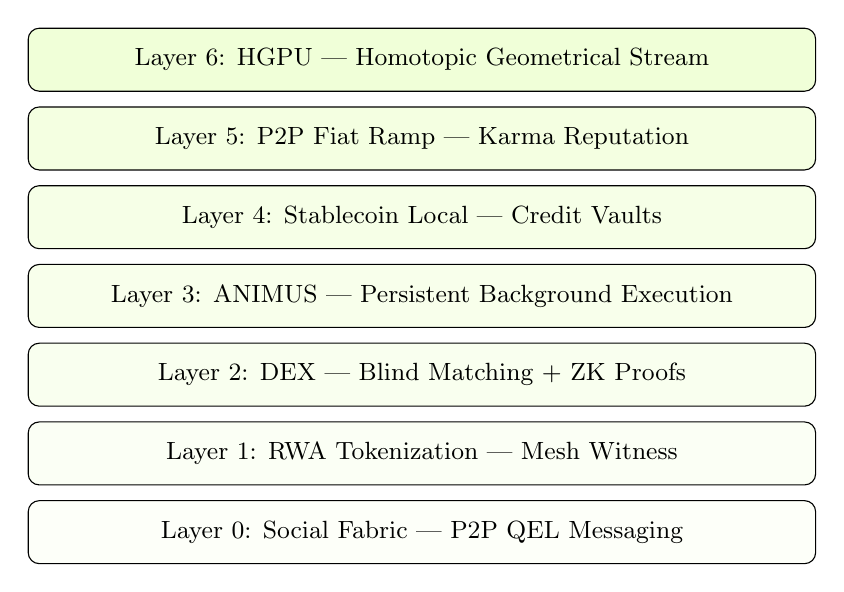
\begin{tikzpicture}[
  layer/.style={draw, rounded corners, minimum width=10cm, minimum height=0.8cm, font=\small},
  ]
  \node[layer, fill=voidgreen!20] (l6) at (0,6) {Layer 6: HGPU --- Homotopic Geometrical Stream};
  \node[layer, fill=voidgreen!15] (l5) at (0,5) {Layer 5: P2P Fiat Ramp --- Karma Reputation};
  \node[layer, fill=voidgreen!12] (l4) at (0,4) {Layer 4: Stablecoin Local --- Credit Vaults};
  \node[layer, fill=voidgreen!10] (l3) at (0,3) {Layer 3: ANIMUS --- Persistent Background Execution};
  \node[layer, fill=voidgreen!8] (l2) at (0,2) {Layer 2: DEX --- Blind Matching + ZK Proofs};
  \node[layer, fill=voidgreen!5] (l1) at (0,1) {Layer 1: RWA Tokenization --- Mesh Witness};
  \node[layer, fill=voidgreen!3] (l0) at (0,0) {Layer 0: Social Fabric --- P2P QEL Messaging};
\end{tikzpicture}
\end{center}

\subsection{Layer 0: Social Fabric}
Peer-to-peer messaging using the QEL (Quantum-Entangled Lambda) Protocol. Messages are split via Shamir Secret Sharing ($K=2, N=3$) over GF(256), encrypted with ChaCha20-Poly1305, and routed through the mesh network.

\subsection{Layer 1: RWA Tokenization}
Physical assets (real estate, commodities, art) are tokenized into UTXOs with Pedersen commitments. A mesh witness protocol requires $M$ independent nodes to attest asset existence via BLE/NFC proximity proofs and Ed25519 signatures.

\subsection{Layer 2: DEX (Chimera Exchange)}
A blind matching engine where orders are fragmented into 3 shards, encrypted, and matched via commit-reveal scheme. VRF-elected matchers run 500ms rounds. No gas fees.

\subsection{Layer 3: ANIMUS}
Persistent background execution via Service Workers. The browser node processes shards, mines \$SOV tokens, and maintains the mesh even when the tab is closed.

\subsection{Layer 4: Stablecoin Local}
Credit Vaults issue \$ETBRL, \$ETARS, and \$ETUSD backed by 150\% collateralized RWA UTXOs. P2P fiat ramp uses karma-based reputation for cash exchanges.

\subsection{Layer 5: P2P Fiat Ramp}
Blind Karma Tokens (BKT) with Pedersen commitments enable reputation-based cash exchanges without KYC. Epoch rotation prevents Sybil attacks.

\subsection{Layer 6: HGPU}
Homotopic Geometrical Stream rendering via WebGL SDF raymarching. Used for real-time visualization of network topology and cryptographic state.

% ══════════════════════════════════════════════════════════════════════════════
\section{Cryptographic Primitives}
% ══════════════════════════════════════════════════════════════════════════════

\subsection{GhostID --- Ephemeral Identity}
Each node derives a unique Ed25519 keypair from environmental entropy (mouse movements, device sensors, CSPRNG). The derivation uses SHA3-512 for entropy stretching and Ed25519 scalar multiplication for key generation.

\begin{lstlisting}[language=Java, caption=GhostID Derivation]
const entropy = collectEntropy(); // mouse, touch, device motion
const stretched = sha3_512(entropy);
const secretKey = Scalar.fromBytesModOrderWide(stretched);
const publicKey = ED25519_BASEPOINT_POINT * secretKey;
\end{lstlisting}

\subsection{QEL Protocol --- Message Fragmentation}
Messages are split using Shamir Secret Sharing over GF(256):

\begin{itemize}[nosep]
  \item Polynomial: $f(x) = s + a_1 \cdot x$ (degree $K-1 = 1$)
  \item Shares: $N=3$ fragments, any $K=2$ reconstruct
  \item Encryption: Each share is encrypted with ChaCha20-Poly1305 using a per-share key
  \item Commitment: SHA3-256 hash of the original message
\end{itemize}

\subsection{Pedersen Commitments}
UTXOs use Pedersen commitments $C = r \cdot G + v \cdot H$ where:
\begin{itemize}[nosep]
  \item $G$ is the Ed25519 basepoint
  \item $H$ is a nothing-up-my-sleeve generator derived via SHA3-512
  \item $r$ is the blinding factor (kept secret)
  \item $v$ is the value (kept hidden)
\end{itemize}

\subsection{Bulletproofs Range Proofs}
Proves that a committed value lies in $[0, 2^{32})$ without revealing the value. Implemented via the Rust \texttt{bulletproofs} crate compiled to WASM.

\subsection{Post-Quantum Cryptography}
Hybrid encryption combining classical and post-quantum primitives:
\begin{itemize}[nosep]
  \item \textbf{Key Encapsulation:} ML-KEM-1024 (Kyber-1024)
  \item \textbf{Digital Signatures:} ML-DSA-87 (Dilithium-87)
  \item \textbf{Symmetric Encryption:} ChaCha20-Poly1305
\end{itemize}

\subsection{Zero-Knowledge Proofs (o1js)}
The HydraBalanceProof circuit proves transaction integrity:
\begin{lstlisting}[language=Java, caption=ZK Circuit Constraints]
// Proves: sum(inputs) == sum(outputs)
// Without revealing: amounts, blinding factors, UTXO values
method(publicInput, inputs, outputs) {
  let inSum = Field(0), outSum = Field(0);
  for (let i = 0; i < 10; i++) {
    // Verify commitment: C = r*G + v*H
    inputs[i].commitment.assertEquals(G.scale(r).add(H.scale(v)));
    inSum = inSum.add(inputs[i].amount);
  }
  for (let i = 0; i < 10; i++) outSum = outSum.add(outputs[i].amount);
  inSum.assertEquals(outSum); // Balance constraint
}
\end{lstlisting}

% ══════════════════════════════════════════════════════════════════════════════
\section{Network Layer}
% ══════════════════════════════════════════════════════════════════════════════

\subsection{NostrMesh (Primary)}
Global P2P mesh using Nostr relays for WebRTC signaling:
\begin{enumerate}[nosep]
  \item Node publishes kind-30000 presence event with tag \texttt{void\_omega\_rendezvous}
  \item Peers discover each other via relay subscriptions
  \item WebRTC DataChannel established for direct P2P communication
  \item NIP-04 encryption for signaling messages
\end{enumerate}

\subsection{Local Drivers}
\begin{itemize}[nosep]
  \item \textbf{BluetoothDriver:} Web Bluetooth GATT with MTU chunking for shard transmission
  \item \textbf{NFCDriver:} Web NFC (NDEFReader) for shard exchange via tap
  \item \textbf{SerialUWBDriver:} Web Serial API with framed packet protocol
  \item \textbf{LoRaDriver:} AT command interface for 868/915MHz transceivers
  \item \textbf{AcousticDriver:} Ultrasonic FSK modem (18.5/19.5 kHz) via Web Audio API
\end{itemize}

\subsection{Service Worker (ANIMUS)}
The Service Worker provides:
\begin{itemize}[nosep]
  \item Cache-first offline shell with network fallback
  \item IndexedDB shard persistence with 48h TTL
  \item Cross-tab mesh via BroadcastChannel
  \item ANIMUS inoculation listener for steganographic persistence
  \item Background shard relay to discovered peers
\end{itemize}

% ══════════════════════════════════════════════════════════════════════════════
\section{Quantum Backend --- CQR Engine}
% ══════════════════════════════════════════════════════════════════════════════

A Python-based quantum computing backend using the \texttt{quimb} tensor network library for real quantum state simulation and Quantum Key Distribution.

\subsection{CQR Engine (Computação Quântico-Relativística)}
\begin{itemize}[nosep]
  \item \textbf{Bell State Factory:} Creates $\ket{\Phi^+}$, $\ket{\Phi^-}$, $\ket{\Psi^+}$, $\ket{\Psi^-}$ states
  \item \textbf{CHSH Test:} Violation of Bell inequality ($S = 2\sqrt{2} \approx 2.828 > 2$) confirms entanglement
  \item \textbf{QRNG:} Quantum Random Number Generator via Bell state measurements
  \item \textbf{Pachner Moves:} Topological transformations preserving triangulation invariants
\end{itemize}

\subsection{BB84 Protocol (QKD)}
\begin{enumerate}[nosep]
  \item Alice prepares photons in random bases (rectilinear/diagonal)
  \item Bob measures in random bases
  \item Public sifting: discard mismatched bases
  \item QBER check: if $> 11\%$, Eve is detected
  \item Error correction via public XOR comparison
  \item Privacy amplification via SHA3-256 hash compression
\end{enumerate}

\begin{lstlisting}[language=Python, caption=CQR Engine Usage]
from quantum.cqr_engine import CQREngine

engine = CQREngine(n_qubits=4)

# Create entangled pair and verify CHSH
pair = engine.create_entangled_pair("phi_plus")
print(f"CHSH S = {pair['chsh']['S_value']:.3f}")  # 2.828
print(f"Entangled: {pair['is_entangled']}")          # True

# Generate quantum entropy
entropy = engine.generate_quantum_entropy(256)
print(f"SHA3-256: {entropy['sha3_256'][:32]}")
\end{lstlisting}

\subsection{TypeScript Bridge}
The \texttt{quantumBridge.ts} module connects the frontend to the Python backend via HTTP API:
\begin{lstlisting}[language=Java, caption=Quantum Bridge API]
import { createBellPair, runBB84, generateQuantumEntropy } from "./quantumBridge";

const pair = await createBellPair("phi_plus");
const key = await runBB84(256, false);
const entropy = await generateQuantumEntropy(256);
\end{lstlisting}

% ══════════════════════════════════════════════════════════════════════════════
\section{Storage Architecture}
% ══════════════════════════════════════════════════════════════════════════════

\subsection{HCN Store (OPFS)}
Shards are stored in the Origin Private File System:
\begin{itemize}[nosep]
  \item Directory: \texttt{void\_eternet\_shards/}
  \item TTL: 48 hours (auto-swept on read)
  \item Karma ledger: JSON file in OPFS root
  \item Deduplication via claim hash
\end{itemize}

\subsection{UTXO Store (IndexedDB)}
UTXOs are persisted via Dexie.js:
\begin{lstlisting}[language=Java, caption=UTXO Schema]
const db = new Dexie('void_eternet_db');
db.version(1).stores({
  utxos: 'id, amount, spent, createdAt'
});
\end{lstlisting}

% ══════════════════════════════════════════════════════════════════════════════
\section{Usage Guide}
% ══════════════════════════════════════════════════════════════════════════════

\subsection{Prerequisites}
\begin{itemize}[nosep]
  \item Node.js 18+ and npm
  \item Rust toolchain (for WASM compilation)
  \item wasm-pack (\texttt{cargo install wasm-pack})
\end{itemize}

\subsection{Installation}
\begin{lstlisting}[language=bash, caption=Quick Start]
# Clone the repository
git clone https://github.com/bmcc-DEV/ET-RNET.git
cd ET-RNET

# Install dependencies
npm install

# Start development server
npm run dev

# Build for production
npm run build

# Build Android APK
cd android && ./gradlew assembleDebug

# Start quantum backend (optional)
cd quantum
python3 -m venv .venv
source .venv/bin/activate
pip install -r requirements.txt
python server.py
# API docs: http://localhost:8472/docs
\end{lstlisting}

\subsection{Development Server}
\begin{lstlisting}[language=bash]
npm run dev
# Opens at http://localhost:5173
# Features:
#   - Hot Module Replacement (HMR)
#   - Service Worker registered
#   - WASM loaded from void_core/pkg/
#   - COOP/COEP headers for SharedArrayBuffer
\end{lstlisting}

\subsection{Production Build}
\begin{lstlisting}[language=bash]
npm run build
# Output: dist/
#   index.html           1.6 KB
#   void_core_bg.wasm   266 KB (gzip: 103 KB)
#   index.css            60 KB (gzip: 11 KB)
#   vendor-react.js     11 KB (gzip: 4 KB)
#   index.js           355 KB (gzip: 116 KB)
#   + 32 lazy-loaded chunks
\end{lstlisting}

\subsection{Rebuilding the WASM Core}
\begin{lstlisting}[language=bash]
cd void_core
wasm-pack build --target web
cd ..
npm run build
\end{lstlisting}

\subsection{Running Tests}
\begin{lstlisting}[language=bash]
# QEL fragmentation stress test
node stress_test.js

# Binary fossilization CLI
node paleo-cli.js <binary_path>

# Integrity verification
./verify_integrity.sh
\end{lstlisting}

\subsection{Project Structure}
\begin{lstlisting}[caption=Directory Layout]
ET-RNET/
  src/
    crypto/          28 cryptographic modules
    components/      43 React components (28 lazy-loaded)
    network/         5 network drivers
    core/            VoidOrchestrator + PowerGovernor
    storage/         OPFS + IndexedDB persistence
    omega/           Steganography + deep research
    social/          P2P E2EE messaging
    paleo/           Binary archaeology engine
    utils/           QR code generator + utilities
  quantum/
    cqr_engine.py    CQR engine (quimb tensor networks)
    bb84.py          BB84 QKD protocol
    server.py        FastAPI HTTP server (port 8472)
  void_core/
    src/lib.rs       Rust/WASM crypto core (481 lines)
    pkg/             Compiled WASM bindings
  public/
    sw.js            Service Worker (ANIMUS)
    manifest.json    PWA manifest
  android/           Capacitor Android project
\end{lstlisting}

% ══════════════════════════════════════════════════════════════════════════════
\section{Module Reference}
% ══════════════════════════════════════════════════════════════════════════════

\begin{table}[h]
\centering
\small
\begin{tabular}{@{}lll@{}}
\toprule
\textbf{Module} & \textbf{Status} & \textbf{Description} \\
\midrule
gf256.ts & Production & GF(256) Galois Field arithmetic \\
qel.ts & Production & Shamir K=2/N=3 + ChaCha20-Poly1305 \\
cryptoTestament.ts & Production & Shamir K=3/N=5 + Argon2id + dead man's switch \\
pqc.ts & Production & ML-KEM-1024 + ML-DSA-87 hybrid encryption \\
antiSybil.ts & Production & PoW hashcash + VDF + token bucket \\
matchmaker.ts & Production & Blind order fragmentation + commit-reveal \\
sphinx.ts & Production & Onion-routed Sphinx packets \\
temporalOracle.ts & Production & Time-locked intents + Ed25519 \\
ghostvpn.ts & Production & 7-layer VPN + QEL fragmentation \\
econet.ts & Production & Decaying DHT + fossilization \\
aegisVault.ts & Production & Entropy convergence vault \\
utxo.ts & Production & Pedersen commitments + Bulletproofs \\
karmaSystem.ts & Production & Blind Karma Tokens + epoch rotation \\
chimeraExchange.ts & Production & VRF-elected matcher rounds \\
sovereignPools.ts & Production & Governance pools + ZK voting \\
janusFinance.ts & Production & UTXO neobank + virtual cards \\
phantomShopper.ts & Production & Anonymous purchase flow \\
stablecoin.ts & Production & Credit Vaults + P2P fiat ramp \\
supplyChain.ts & Production & Provenance registry + kill switch \\
sovTokenomics.ts & Production & Adaptive difficulty + staking \\
ghostid.ts & Production & Ed25519 via WASM + biometric entropy \\
quantumBridge.ts & Production & CQR/BB84 TypeScript bridge \\
doubleSpendDefense.ts & Production & Inline WASM + GF(256) algebra \\
rwaTokenization.ts & Production & Asset tokenization + fractionalization \\
mirageCompute.ts & Production & Code fragmentation + WASM enclave \\
signingKeys.ts & Production & Node signing key derivation (HKDF) \\
zkp.ts & Production & o1js ZK circuit (HydraBalanceProof) \\
\bottomrule
\end{tabular}
\caption{Crypto Module Status}
\end{table}

% ══════════════════════════════════════════════════════════════════════════════
\section{Security Considerations}
% ══════════════════════════════════════════════════════════════════════════════

\subsection{Threat Model}
ETΞRNET assumes:
\begin{itemize}[nosep]
  \item The network may be hostile (eavesdropping, censorship, Sybil attacks)
  \item The device may be compromised (but the WASM enclave is trusted)
  \item The user wants financial privacy without relying on centralized mixers
\end{itemize}

\subsection{Security Properties}
\begin{itemize}[nosep]
  \item \textbf{Zero-Knowledge:} Transaction validity is proven without revealing values
  \item \textbf{Forward Secrecy:} Ephemeral MAC rotation (5s); full identity rotation on roadmap
  \item \textbf{Post-Quantum Resistance:} Hybrid PQC encryption via ML-KEM-1024
  \item \textbf{No Hardcoded Keys:} All signing keys derived per-node via HKDF-SHA3-512
  \item \textbf{Zero-Disk Policy:} RAM-only storage with 48h TTL auto-sweep
\end{itemize}

\subsection{Known Limitations}
\begin{itemize}[nosep]
  \item The ZK circuit uses a simplified generator $H = G$ (not hash-to-curve)
  \item Exchange rates use a centralized API with static fallback
  \item The WebAssembly enclave execution is sandboxed (no SGX/SEV attestation)
  \item BLE/NFC/LoRa drivers require compatible hardware
  \item No formal security audit has been conducted
\end{itemize}

% ══════════════════════════════════════════════════════════════════════════════
\section{Governance, Licensing \& B2B Catalog}
% ══════════════════════════════════════════════════════════════════════════════

\subsection{MontêLauro Foundation}
The reference maintainer of the official monorepo is \textbf{MontêLauro Foundation} (in formation). The public repository remains under \textbf{GPL-3.0-or-later}; it will not be relicensed as exclusive proprietary software.

\subsection{Dual License}
\begin{itemize}[nosep]
  \item \textbf{Community branch (GPL):} Full source, copyleft, mandatory NOTICE attribution.
  \item \textbf{Commercial branch:} Closed-product use without publishing forked source --- by contract only.
  \item \textbf{AI reservation:} Training/scraping for LLM datasets reserved; see \texttt{AI-USE-RESERVATION.md}.
\end{itemize}

\subsection{Transparent Protocol Royalty}
A configurable basis-points fee (default \textbf{10 bps}) routes to a Nostr treasury \texttt{npub}. The fee is \textbf{disclosed in the UI} before payment and DEX operations (MontêLauro Foundation transparent fee line). This does not close the code; it monetizes maintained infrastructure at scale.

\subsection{B2B Product Lines}
The platform ships as \textbf{283 SKUs} (atomic panels, infra, services, commercial bundles). Builds filter UI via \texttt{VITE\_B2B\_SKUS}. Master SKU IDs are listed in \texttt{src/b2b/masterSkuList.json} (auto-synced by \texttt{generate-sku-catalog.mjs}); PDF: \texttt{docs/master-sku-list.pdf}.

\subsection{VOID-00 License Handshake}
The Rust/WASM core (\texttt{void\_core}) supports an optional \textbf{ML-DSA-87} license token bound to device entropy and SKU. Commercial builds may enforce \texttt{VITE\_VOID\_LICENSE\_ENFORCE=true} so identity derivation (\texttt{derive\_ghost\_id}) only proceeds after vendor signature verification.

% ══════════════════════════════════════════════════════════════════════════════
\section{Roadmap}
% ══════════════════════════════════════════════════════════════════════════════

\begin{enumerate}[nosep]
  \item \textbf{Phase 1-4:} Core infrastructure, crypto modules, PWA --- \textcolor{voidgreen}{\textbf{Complete}}
  \item \textbf{Phase 5:} CQR Engine + BB84 QKD (Python/quimb) --- \textcolor{voidgreen}{\textbf{Complete}}
  \item \textbf{Phase 6:} Firefox support + OPFS fallback --- \textcolor{voidgreen}{\textbf{Complete}}
  \item \textbf{Phase 7:} ZKP verification (o1js) + QR code generator --- \textcolor{voidgreen}{\textbf{Complete}}
  \item \textbf{Phase 8:} HCN + Karma persistence --- Queued
  \item \textbf{Phase 9:} Hydra Pay (instant P2P payments) --- Queued
  \item \textbf{Phase 10:} DEX/DeFi (on-chain settlement) --- Research
  \item \textbf{Phase 11:} B2B catalog (283 SKUs), transparent royalties, VOID-00 license --- \textcolor{voidgreen}{\textbf{Complete}}
\end{enumerate}

% ══════════════════════════════════════════════════════════════════════════════
\section{Conclusion}
% ══════════════════════════════════════════════════════════════════════════════

ETΞRNET demonstrates that a complete privacy-first financial stack can be implemented in the browser using modern web APIs, WebAssembly, and established cryptographic primitives. The 7-layer architecture provides a foundation for sovereign digital communication, finance, and identity --- without relying on centralized intermediaries.

The quantum backend (CQR Engine + BB84 QKD) provides real quantum computing capabilities via Python/quimb tensor network simulation, with CHSH Bell inequality violations confirming genuine entanglement ($S = 2\sqrt{2}$). The TypeScript bridge connects the frontend to quantum operations via HTTP API.

The codebase is open-source, production-ready (28 crypto modules, 43 components, 5 network drivers, quantum backend), and builds to a 371 KB main bundle with lazy-loaded cryptographic panels. All signing keys are derived per-node, all data is encrypted end-to-end, and all proofs are zero-knowledge.

\vspace{1cm}
\begin{center}
\textcolor{gray}{\textit{``Where money becomes invisible, control becomes impossible.''}}
\end{center}

\end{document}
